\documentclass[11pt,psfig]{article}
\usepackage{epsfig}
\usepackage{times}
\usepackage{amssymb}
\usepackage{float}

\newcount\refno\refno=1
\def\ref{\the\refno \global\advance\refno by 1}
\def\ux{\underline{x}}
\def\uw{\underline{w}}
\def\bw{\underline{w}}
\def\ut{\underline{\theta}}
\def\umu{\underline{\mu}} 
\def\bmu{\underline{\mu}} 
\def\be{p_e^*}
\newcount\eqnumber\eqnumber=1
\def\eq{\the \eqnumber \global\advance\eqnumber by 1}
\def\eqs{\eq}
\def\eqn{\eqno(\eq)}

 \pagestyle{empty}
\def\baselinestretch{1.1}
\topmargin1in \headsep0.3in
\topmargin0in \oddsidemargin0in \textwidth6.5in \textheight8.5in
\begin{document}
\setlength{\parskip}{1.2ex plus0.3ex minus 0.3ex}


\thispagestyle{empty} \pagestyle{myheadings} \markright{G}



\title{CS 266 Homework 7}
\author{Zachary DeStefano, PhD Student, 15247592}
\date{Due Date: May 29, 2014}

\maketitle

\vfill\eject

\section*{Problem 7.7}
This is false. There are cases we can construct where the beach line breakpoints would move upward. Let's take the example of two points that are on a diagonal line and we construct the Voronoi diagram for just those two points. When the second point is reached, there will be two breakpoints from the two intersections of the parabolas and one of the breakpoints will move upward while the other moves downward.

\begin{figure}[H]
\centering
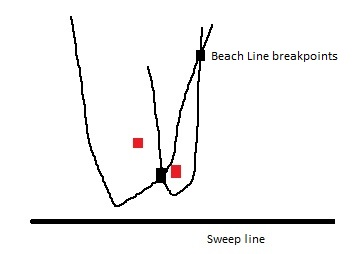
\includegraphics[height=2.5in]{hw7prob1diagram.jpg}
\caption{Beach Line example. The top breakpoint will move up while the bottom one will move down.}
\end{figure}

\section*{Problem 7.11}

Here is the algorithm:\\
1. Compute the Voronoi Diagram\\
2. For the cell of p:\\
Find perpendicular distance to each edge of p\\
Figure out which is closer and the corresponding point is the closest one to p\\
\\
Running time:\\
There are n cells\\
There are $O(n)$ edges total since the storage required is $O(n)$\\
thus the checking step takes a total of $O(n)$ time. \\
Computing the Voronoi Diagram will take $O(n \cdot log(n))$ time. \\
Total running time is thus $O(n \cdot log(n))$

\section*{Problem 9.11}

\subsection*{Part a}
Suppose there are two points $p$ and $q$ whose edge is in the EMST but whose edge is not in the Delaunay Triangulation. Since it is not in the Delaunay Tringulation, there is at least one point $r$ between $p$ and $q$\\
Now, take out $r$ and separate the graph into two sets of vertices, one with $p$ and one with $q$. \\
Compute the EMST of the two sets. We now have to add back in $r$ and join the sets via edges. \\
The logical choice would be $pr$,$rq$ however we also said that there was a line between $p$ and $q$ in the EMST, thus those are connected. \\
WLOG assume $r$ is closer to $p$ than $q$, then the next edge would be $pr$. \\
We are thus forced to have our edges be $pq$ and $pr$\\
By what was said above, we know that $pq$ has greater weight that $rq$. \\
Thus the EMST we want to construct will have less weight than the EMST we would be forced to construct with the initial condition. 
We thus did not have an EMST to begin with, a contradiction.

\begin{figure}[H]
\centering
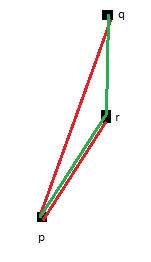
\includegraphics[height=2in]{hw7prob2diagram.jpg}
\caption{The Points $p,q,r$. Green are the good edges. Red that are edges from the faulty scenario}
\end{figure} 

\subsection*{Part b}
Here is the algorithm:\\
1. Compute the Delaunay Triangulation. \\
2. Apply Prims's algorithm to the graph derived from the triangulation to get the EMST.\\
\\
Running time:\\
Delaunay Triangulation takes $O(n \cdot logn)$ time.\\
There are $O(n)$ edges and $O(n)$ vertices, thus Prim's will take $O(n \cdot logn)$ time. \\
The total running time is thus $O(n \cdot logn)$\\

\newpage

\section*{Problem 9.17}

If we take a quadrilateral that points inward, then we can construct a case where the Delaunay triangulation will have greater weight than the minimum weight triangulation. The Delaunay Triangulation could end up choosing a high weight edge that you would not want to include in the minimum weight triangulation. 

\begin{figure}[H]
\centering
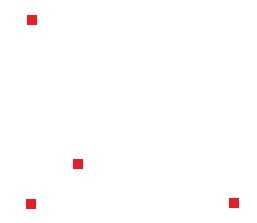
\includegraphics[height=2.5in]{hw7prob3diagram1.jpg}
\caption{The Four Points to Triangulate}
\end{figure}

\begin{figure}[H]
\centering
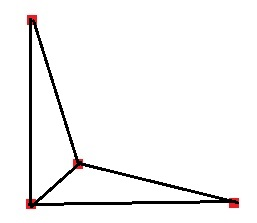
\includegraphics[height=2.5in]{hw7prob3diagram2.jpg}
\caption{The Minimum Weight Triangulation}
\end{figure}

\begin{figure}[H]
\centering
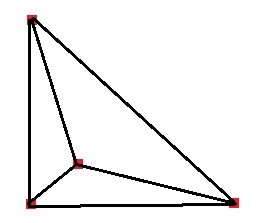
\includegraphics[height=2.5in]{hw7prob3diagram3.jpg}
\caption{The Delaunay Triangulation}
\end{figure}

\end{document}








